\subsection{Realización del esquema de almacenamiento comprimido con Blosc}

El punto de entrada del desarrollo es la clase \texttt{QuantumRegister}, que conserva la
interfaz de uso del registro cuántico y delega las operaciones sobre el vector de estado
en un backend que satisface la interfaz \texttt{IStateBackend}. En el repositorio
intervenido, esa interfaz abstrae operaciones de inicialización
(\texttt{initZero}, \texttt{initBasis}, \texttt{loadAmplitudes}), operaciones de
exportación del estado, acceso elemental
(\texttt{amplitude}, \texttt{setAmplitude}) y aplicación de compuertas, además de dos
operaciones opcionales para delimitar lotes mutables
(\texttt{beginOperationBatch}/\texttt{endOperationBatch}). Esta abstracción fue clave
para sustituir el almacenamiento denso sin cambiar la API visible para los algoritmos.

Sobre esa interfaz se implementó \texttt{BloscStateBackend}, que constituye la
realización concreta del almacenamiento comprimido. La clase mantiene el número de
qubits y estados, la configuración resuelta, un \texttt{ChunkLayout}, un
\texttt{ChunkCache}, un \texttt{BloscCodec}, un buffer auxiliar de lectura
(\texttt{ioScratch\_}), la profundidad de lote (\texttt{batchDepth\_}) y un
\textit{workspace} reutilizable para compuertas generales. Su responsabilidad central
no es ``comprimir'' en abstracto, sino coordinar el ciclo completo de cada acceso:
determinar el bloque implicado, recuperar su versión descomprimida si hace falta,
entregar punteros mutables a las amplitudes afectadas, marcar suciedad y decidir
cuándo persistir la actualización de vuelta al almacenamiento comprimido.

La compresión efectiva se delega en \texttt{BloscCodec}, que encapsula la API de
Blosc2 y mantiene el super-chunk comprimido. Este componente valida parámetros como
\texttt{chunkStates}, \texttt{gateCacheSlots}, \texttt{clevel} y \texttt{nthreads},
crea el contenedor comprimido, anexa bloques en la inicialización y actualiza bloques ya
existentes en las escrituras. Además reutiliza un contexto de compresión y un buffer
\textit{scratch} para evitar recrear recursos del códec en cada actualización, lo cual
reduce parte de la sobrecarga de recompresión.

\begin{figure}[H]
    \centering
    \caption{Diagrama de clases de la implementación del backend comprimido basado en Blosc2.}
    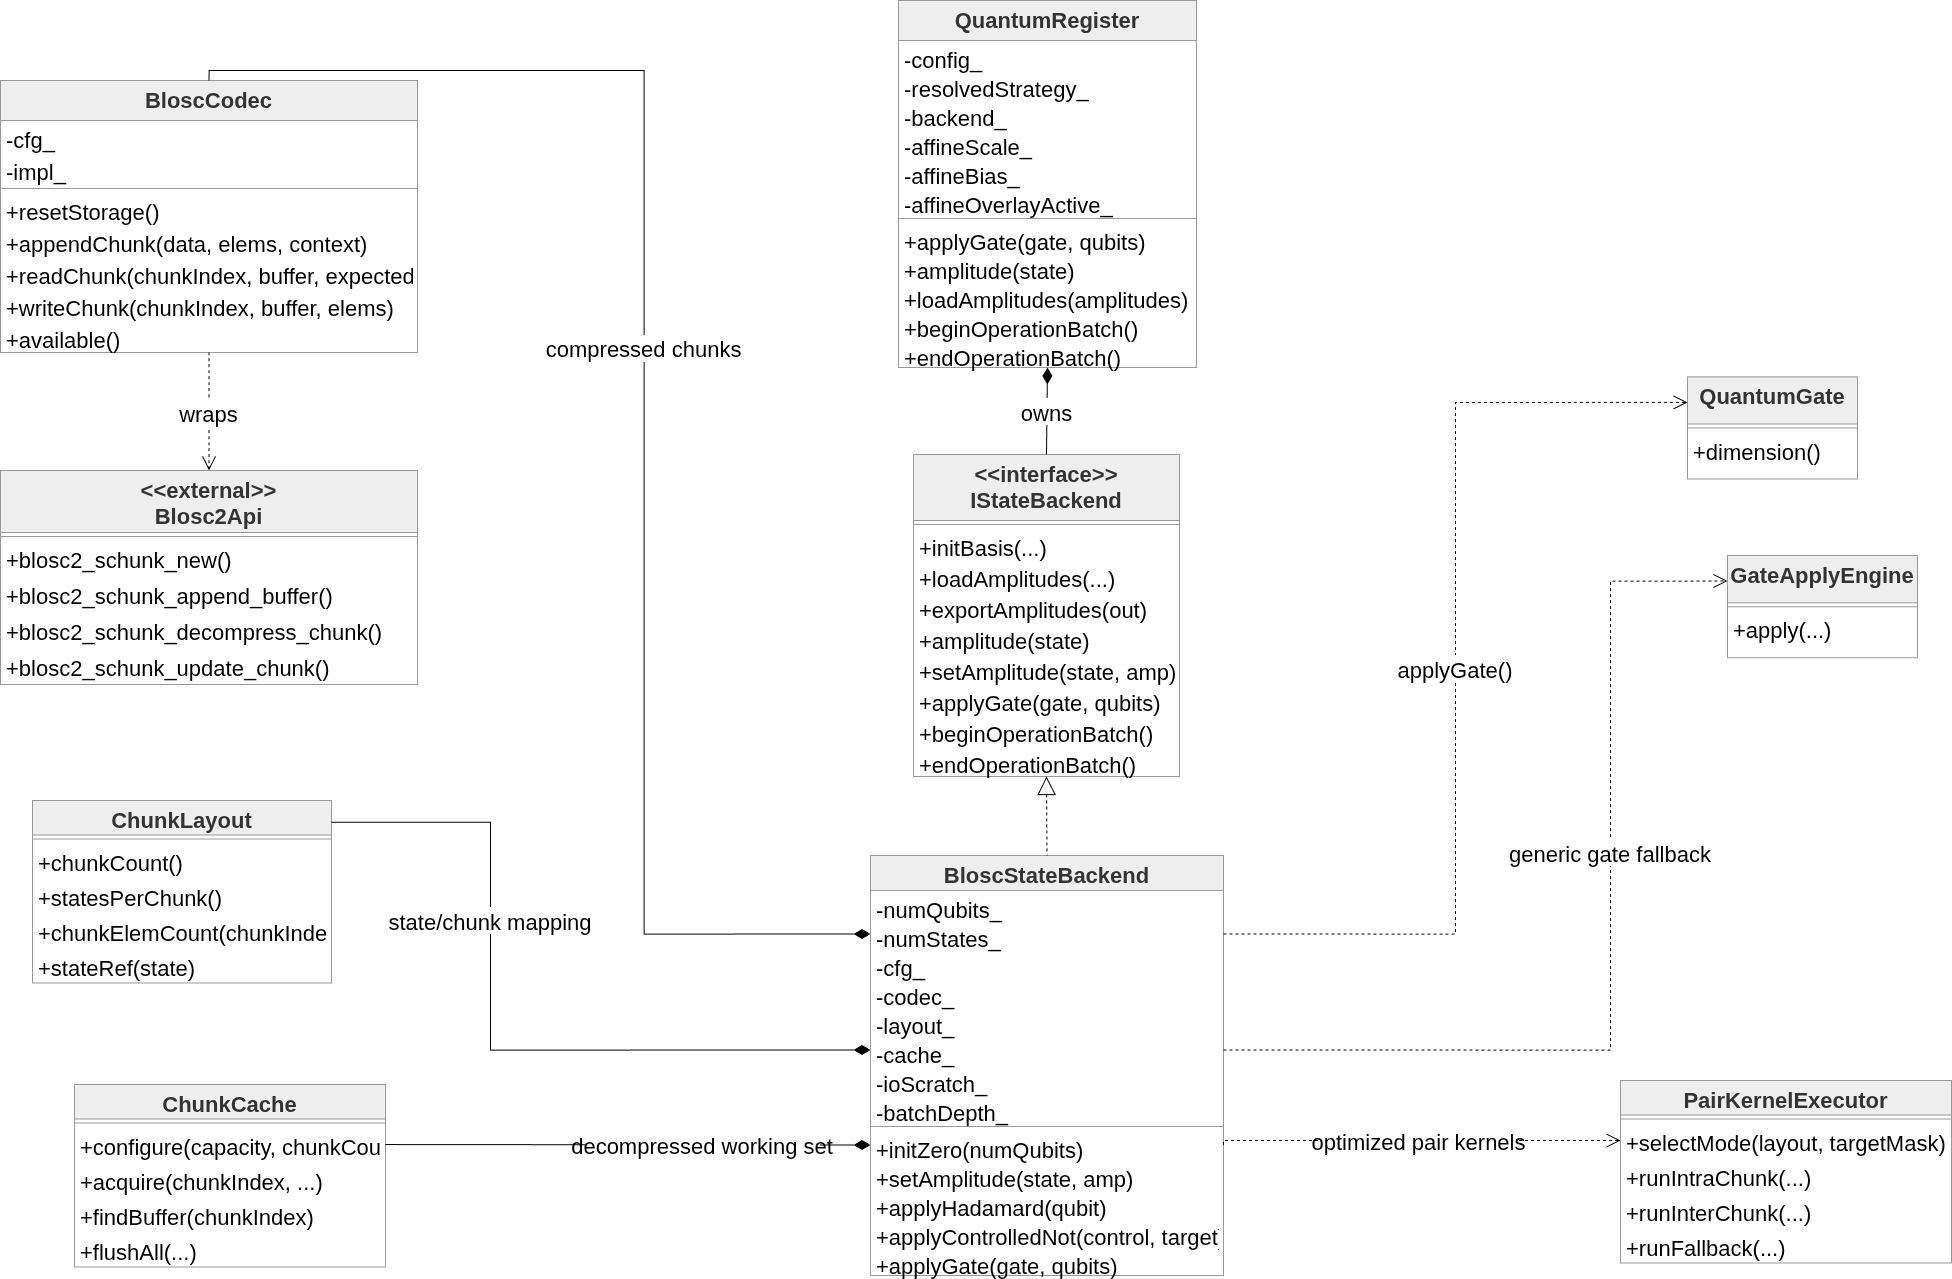
\includegraphics[width=1\linewidth]{images/class-diagram.png}
    \label{fig:impl_class_diagram}
\end{figure}

La figura \ref{fig:impl_class_diagram} resume la organización general de esta
implementación. En ella se observa la relación entre el registro cuántico, la interfaz de
backend, la realización basada en Blosc, los componentes auxiliares de layout y caché, y
los mecanismos de ejecución de compuertas.

En conjunto, esta organización permite que la compresión se integre como una
responsabilidad propia de la capa de almacenamiento, y no como una operación aislada
externa al flujo del simulador. Lo implementado no es un posprocesamiento del vector,
sino un backend que mantiene la representación comprimida como estado nativo de
ejecución.
